\par{The internal kernel is the dominant kernel in this implementation of the LU decomposition. 
    It accounts for the majority of computation time. It operates on a larger amount of data 
    than each of the other kernels and is also very inefficient, in spite of a high level of parallelism.}

\begin{figure}[!h]
    \centering
    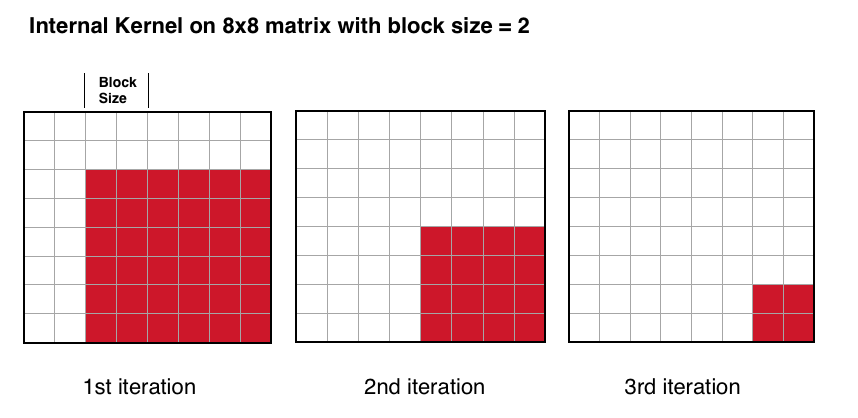
\includegraphics[width=0.6\textwidth]{figures/InternalKernel2.png}
    \caption{Internal kernel algorithm on 8x8 matrix with block size = 2.}
    \label{InternalKernel2}
\end{figure}

\par{The first instance of the internal kernel operates on the 1st portion of the matrix shown in figure \ref{InternalKernel2}. 
    All kernels are enqueued multiple times, so, the next execution of the kernel will operate on 
    a portion of the matrix that has been decreased by block size in each dimension.}

\par{Table \ref{tab:lu3} summarises the relevant parameters.}

\begin{table}[!h]
    \centering
    \begin{tabular}{| l | l | l | l |}
    \hline
    \emph{Block Size} & \emph{Data Block / Work Group} & \emph{Starting Number of Work Groups} & \emph{\#Work-Items / Work-Group} \\ \hline
    2 & 3x(2x2) & 4,190,209 & 4 \\ \hline
    4 & 3x(4x4) & 1,046,529 & 16 \\ \hline
    8 & 3x(8x8) & 261,121 & 64 \\ \hline
    16 & 3x(16x16) & 65,025 & 256 \\ \hline
    32 & 3x(32x32) & 16,129 & 1024 \\ \hline
    64 & 3x(64x64) & 3,969 & 4096 \\ \hline
    \end{tabular}
    \caption{Internal Kernal Summary.}
    \label{tab:lu3}
\end{table}

\par{The first thing to note is that the number of work-groups is very high, which means
    that the algorithm is exploiting the available parallelism in the Xeon CPU and Xeon Phi relatively well. 
    There are almost always enough work-groups to fill the available hardware threads. 
    As a result, the number of GFLOPS is significantly higher in executions of the internal 
    kernel than in executions of the other kernels, which do not exploit the parallelism to the same extent. 
    This is a clear demonstration of the performance gains possible from correct utilisation of the available hardware. 
    Table \ref{tab:lu4} compares the number of GFLOPS between executions of the diagonal 
    kernel and the internal kernel on the Xeon CPU.}

\begin{table}[!h]
    \centering
    \begin{tabular}{| l | l | l | l |}
    \hline
    \emph{Block Size} & \emph{Diagonal} & \emph{Internal} \\ \hline
    2 & 0.00005 & 8.40286 \\ \hline
    4 & 0.00057 & 16.53493 \\ \hline
    8 & 0.00172 & 26.83808 \\ \hline
    16 & 0.03334 & 29.94455 \\ \hline
    32 & 0.11905 & 28.50387 \\ \hline
    64 & 0.30937 & 26.86795 \\ \hline
    \end{tabular}
    \caption{Comparison of GFLOPS - Diagonal v Internal Kernels.}
    \label{tab:lu4}
\end{table}

\par{In spite of this, the internal kernel is clearly not an optimal algorithm. 
    When the work-groups are first enqueued, the kernels operate on a very large block of data. 
    In the next iteration of the loop, the kernels operate on almost the same block of data, 
    albeit decreased by block size in each dimension. Thus, the kernel is operating multiple times 
    on almost the same blocks of data. There is an enormous amount of time spent carrying out redundant 
    calculations and reloading the same data from global to local memory.}

\par{The total number of floating point operations that the internal kernel executions perform 
    reduces with the block size, since the number of redundant operations reduces.}

\par{Figure \ref{InternalKernel1} below shows the total computation times for the internal kernel on each of the three devices.}

\begin{figure}[!h]
    \centering
    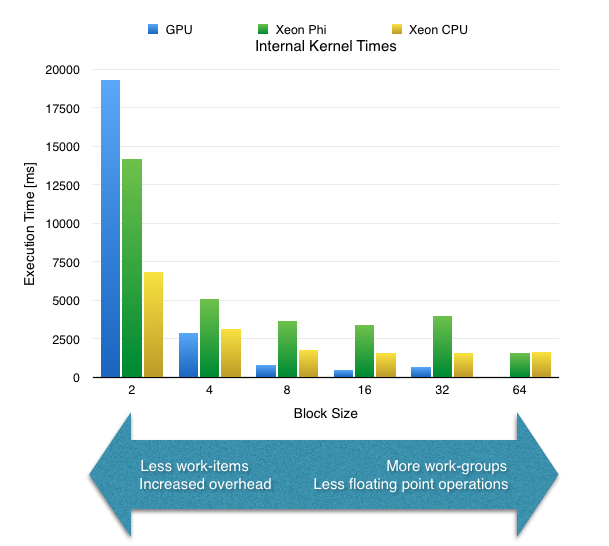
\includegraphics[width=0.6\textwidth]{figures/InternalKernel1.png}
    \caption{4096x4096 Internal Kernel Times.}
    \label{InternalKernel1}
\end{figure}

\par{The above graph highlights some interesting points. It is clear to see that when 
    the number of work-items is minimised (block size 2), the GPU offers the worst performance. 
    As mentioned previously, optimal performance on the GPU is achieved with a large number of 
    work-items per work-group. Significant performance improvements are seen on the GPU 
    as the number of work- items per work-group increases.}

\par{Another interesting point to note is that, as the block size increases, 
    the performance of the Xeon CPU and Xeon Phi improves. This is not only due 
    to the decrease in floating point operations, but also due to the increase in
    work-items per work-group whilst still maintaining a large number of work-groups. 
    Intel’s SDK for OpenCL Applications states that:}

\par{\emph{``To reduce the overhead of maintaining a work-group, create work-groups that
    are as large as possible. Still there should be a sufficient number of work-groups."}}

\par{The internal kernel satisfies these conditions for large block sizes and the performance improves as a result.}
